\documentclass[palatino]{apuntes}

\title{Práctica 4}
\author{Daniel Ruiz Mayo, Alberto Javier Parramón, Víctor de Juan Sanz}
\date{05/2016}

\usepackage{multicol}


% Paquetes adicionales

% --------------------

\begin{document}
\pagestyle{plain}
\maketitle

\chapter{Recomendación}
\section{Consideraciones generales}

	La implementación se basa en matrices de floats. 
	%
	El rendimiento de esta implementación es menor tanto en memoria como en rendimiento (porque almacenamos ceros innecesarios) que las implementaciones nuestros compañeros para el problema resuelto.
	%
	Sin embargo, esta implementación hace muy sencillo trabajar, ya que basta hacer productos escalares en la mayoría de los casos. 
	%
	También es muy sencillo calcular las similitudes.
	
	El problema de la necesidad de definir el tamaño de la matriz al crearla ha sido solucionado  creándola con un tamaño inicial y modificándolo dinámicamente según haga falta.

	También hemos necesitado 2 maps de "índice del elemento" a "índice en la matriz". 
	%
	Esto se debe a que el primer usuario en el fichero de valoraciones es el 75 
	%
	y debe corresponderse con la primera columna de la matriz de usuarios.

	Esta implementación puede no haber sido la correcta para afrontar este problema porque no todos los usuarios han visto todas las películas, lo que provoca muchos ceros. 
	%
	Si la proporción de las películas que ha visto cada usuario fuera cercano a 1, esta implementación escalará mucho mejor que las demás, tanto en memoria como en rendimiento.
	

	Pensamos que al utilizar una librería externa para trabajar con matrices, ésta incorporaría optimizaciones. 
	%
	La librería utilizada ha sido \href{http://ejml.org/wiki/index.php?title=Main_Page}{ejml} (Efficient Java Matrix Library) que no da soporte a matrices dispersas.
	%
	Debido a falta de tiempo no hemos cambiado la librería utilizada a una que incluya soporte con optimizaciones para matrices dispersas.
	%
	Debido al diseño modular de la implementación, no sería difícil modificar la librería utilizada.
	%
	Sólo habría que rehacer el encapsulado de la clase \textit{Matrix.java} para que utilice las funciones y los tipos de datos de la otra librería escogida.



\section{Ejercicio 1}

	Para este ejercicio se ha implementado Rocchio.
	%
	Gracias a la implementación escogida con matrices, basta calcular un producto de matrices.
	%
	La similitud escogida ha sido el coseno.
	
	Lo hemos implementado de tal manera que los centroides de todos los usuarios se calculan al principio y así cada recomendación es más rápida.
	



\section{Ejercicio 2}

	Para este ejercicio se ha implementado KNN- colaborativo orientado a usuario. 
	%
	La similitud aplicada a los usuarios es la del coseno.

 	En esta matriz tenemos los usuarios en las filas y en las columnas, las películas. 
 	%
 	Guardamos en cada celda el rating, de igual manera a los ejemplos realizados en clase.

 	Para la elaboración del algoritmo se han usado las fórmulas vistas en clase para KNN-colaborativo orientado a usuario con la similitud indicada anteriormente.

 	Tenemos una función de predicción, \textit{rank} , que dado un usuario y un item devuelve la predicción de cuanto le va a gustar ese ítem al usuario.
 	%
  	También hemos implementado una función \textit{recommend} que recomienda un número de películas dado como argumento.


\section{Ejercicio 3}

   En el primer ejercicio hemos usado Rocchio y con este método sólo podemos conocer un ranking pero no predecir un rating. 
   %
   Por este motivo sólo podemos evaluar KNN-colaborativo orientado a usuario (el elegido en el ejercicio 2).

   Nuestra implementación consiste en duplicar la matriz del ejercicio 2, reemplazar un 20\% de ratings por un 0 en la matriz  en los sitios que el rating sea distinto de 0, es decir, de los que estan puntuados, y predecir estos valores.
   %
   Posteriormente aplicamos la fórmula de MAE y de MRSE y estos son los resultados:

   
   	\begin{table}[h!]
   		\centering
		\begin{tabular}{ccc}
			Vecinos  &  MAE &  MRSE \\
			25 & 0.78 & 1.03 \\
			50 & 0.74 & 0.96 \\
			75 & 0.72 & 0.94 \\
			100 & 0.72 & 0.94 \\
			250 & 0.70 & 0.90 \\
			500 & 0.69 & 0.90 
		\end{tabular}
		\caption{Resultados de la evaluación}
	\end{table}





\chapter{Redes sociales}

\section{Ejecución}

Para ejecutar esta parte de la práctica únicamente hay que poner como directorio de trabajo el directorio de la práctica bmi1414-p4-12. Posteriormente habrá que ejecutar la clase AnálisisGrafos.java. El método main de dicha clase calcula todas las métricas que se piden en el enunciado y va informando paso por paso de las acciones realizadas. El proceso entero puede tardar cerca de 80 minutos.

Las gráficas se generan con R, los scripts R y las gráficas generados también vienen adjuntados en la práctica en el directorio $resultados/grados$, $resultados/prgrado$ y $resultados/betweenessgrado$.

Así mismo las salidas por fichero que se piden se encuentran en el directorio $resultados$.


\section{Análisis}


\begin{table}[h!]
\caption{TOP 10 PageRank de nodo}
\centering
\begin{tabular}{ccc}
small2&3&0.2338\\
small1&6&0.1084\\
small2&1&0.0958\\
small2&2&0.0958\\
small2&4&0.0958\\
small2&5&0.0958\\
small2&6&0.0958\\
small2&7&0.0958\\
small2&8&0.0958\\
small2&9&0.0958\\
\end{tabular}
\end{table}



\begin{table}[h!]
\centering
\caption{TOP 10 coeficiente de clustering de nodo}
\begin{tabular}{ccc}
fb&865&1.0\\
fb&868&1.0\\
fb&873&1.0\\
fb&877&1.0\\
fb&887&1.0\\
fb&888&1.0\\
fb&899&1.0\\
twitter&envasados&1.0\\
fb&854&1.0\\
fb&851&1.0\\
\end{tabular}
\end{table}



\begin{table}[h!]
\centering
\caption{TOP 10 \textbf{arraigo} de arcos}
\begin{tabular}{ccc}
twitter & e\_463148-neilepstein-neilepstein  &  1.2\\
twitter & e\_267707-beaulebens-beaulebens  &  1.036\\
fb & e\_644312-2824-3091  &  1.0\\
fb & e\_607521-3911-3700  &  1.0\\
fb & e\_607635-3849-3444  &  1.0\\
fb & e\_607522-3864-3813  &  1.0\\
fb & e\_560900-659-627  &  1.0\\
fb & e\_575932-135-309  &  1.0\\
fb & e\_560295-3127-3074  &  1.0\\
fb & e\_560369-195-78  &  1.0\\
\end{tabular} 
\end{table} 



\begin{table}[h!]
\centering
\caption{Coeficiente de \textbf{clustering} global de los grafos}
\begin{tabular}{cc}
small1 & 0.564\\
small2 & 0.624\\
twitter & 0.273\\
fb & 0.544\\
erdos & 0.250\\
barabasi  &0.146\\
\end{tabular}
\end{table}




\begin{table}[h!]
\centering
\caption{Coeficiente de \textbf{asortatividad} de los grafos}
\begin{tabular}{cc}
small1 & -0.21\\
small2 & -0.33\\
twitter & -0.15\\
fb & 0.63\\
erdos & -0.002\\
barabasi & -0.41
\end{tabular}
\end{table}


\newpage

\textbf{Número de puentes locales: }

Como anécdota comentar que al encontrar puentes locales también hemos encontrado parejas de nodos comunicados entre sí e incomunicados del resto del grafo, por definición son puentes locales pero son muchos más raros que estos. Vemos aquí los puentes locales de cada red:

\begin{table}[h!]
\centering
\begin{tabular}{cc}
small1&5\\
small2&0\\
twitter&6843\\
fb&712\\
erdos&0\\
barabasi&1235\\
\end{tabular}
\end{table}

\newpage

\textbf{Paradoja de la amistad}
Para ver si se cumple la paradoja de la amistad hemos utilizado la siguiente fórmula:
$$ AVG_u g(u) \leq AVG_{u\rightarrow v}g(v) $$

\begin{table}[h!]
\centering
\caption{Paradoja de la amistad}
\begin{tabular}{ccc}
small1 & Sí se cumple la paradoja de la amistad & 2.769 <= 2.910\\
small2 & Sí se cumple la paradoja de la amistad & 3.555 <= 4.481\\
twitter & Sí se cumple la paradoja de la amistad & 92.212 <= 237.102\\
fb & Sí se cumple la paradoja de la amistad & 42.557 <= 56.071\\
erdos & Sí se cumple la paradoja de la amistad & 499.713 500.481\\
barabasi & Sí se cumple la paradoja de la amistad & 4.761 <= 43.269\\
\end{tabular}
\end{table}



\newpage
\subsection{Representación gráfica de la distribución de grado }



\begin{figure}[h!]
	\centering
	\begin{minipage}[b]{0.4\textwidth}
		\caption{Twitter}
		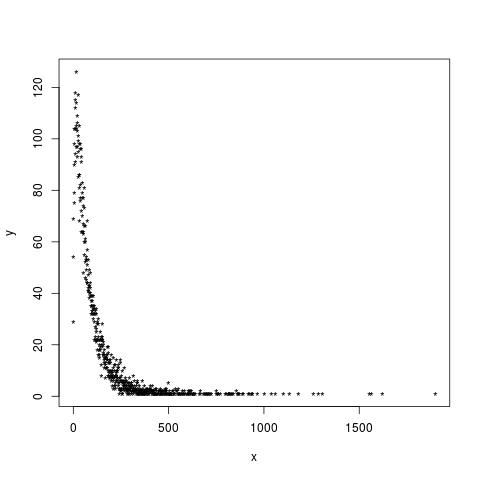
\includegraphics[scale=0.45]{img/twitter_grado}
	\end{minipage}
	\hfill
	\begin{minipage}[b]{0.4\textwidth}
		\caption{Facebook}
		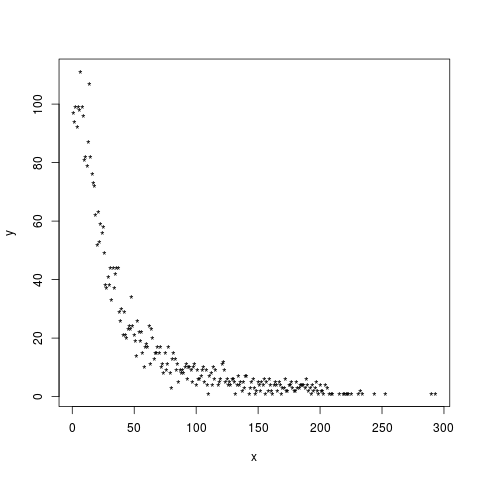
\includegraphics[scale=0.45]{img/fb_grado}
	\end{minipage}
\end{figure}

\begin{figure}[h!] 
\centering 
\begin{minipage}[b]{0.4\textwidth}
	\caption{Barabasi}
	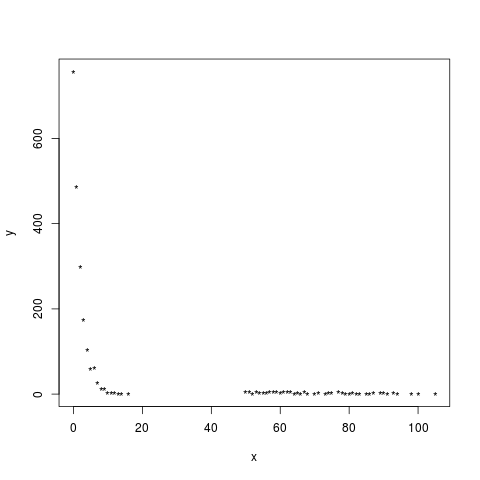
\includegraphics[scale=0.45]{img/barabasi_grado}
\end{minipage}
\hfill
\begin{minipage}[b]{0.4\textwidth}
	\caption{Erdos}
	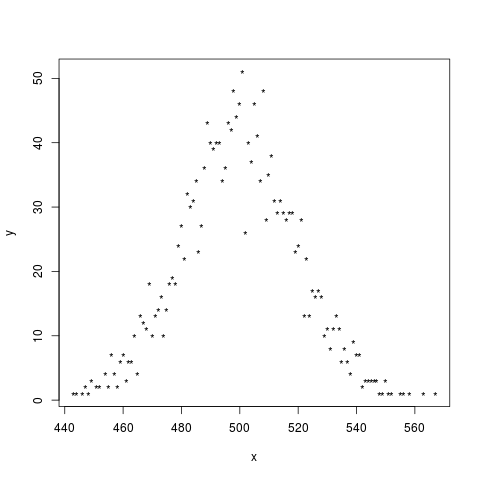
\includegraphics[scale=0.45]{img/erdos_grado}
\end{minipage}
\end{figure} 


\newpage
\subsection{Representación gráfica del grado frente al PageRank }


\begin{figure}[h!] 
\centering 
\begin{minipage}[b]{0.4\textwidth}
	\caption{small1}
	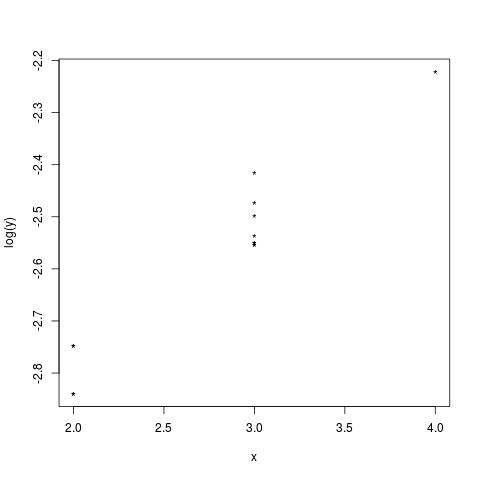
\includegraphics[scale=0.45]{img/small1_grado-pr}
\end{minipage}
\hfill
\begin{minipage}[b]{0.4\textwidth}
	\caption{small2}
	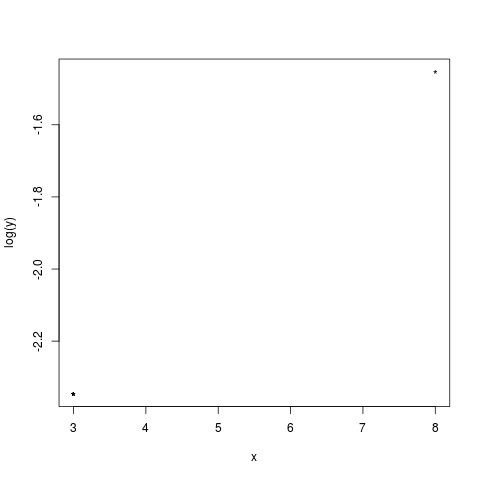
\includegraphics[scale=0.45]{img/small2_grado-pr}
\end{minipage}
\end{figure} 


\begin{figure}[h!] 
\centering 
\begin{minipage}[b]{0.4\textwidth}
	\caption{Twitter}
	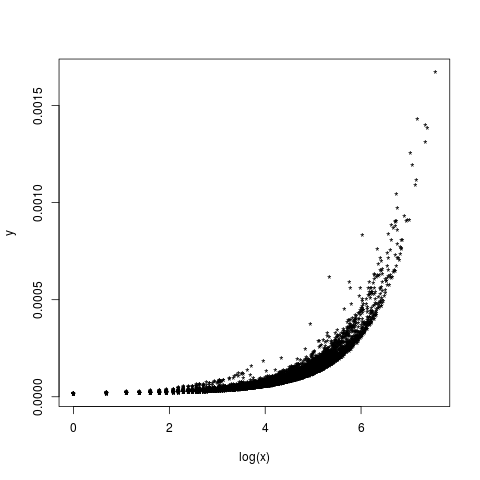
\includegraphics[scale=0.45]{img/twitter_grado-pr}
\end{minipage}
\hfill
\begin{minipage}[b]{0.4\textwidth}
	\caption{Facebook}
	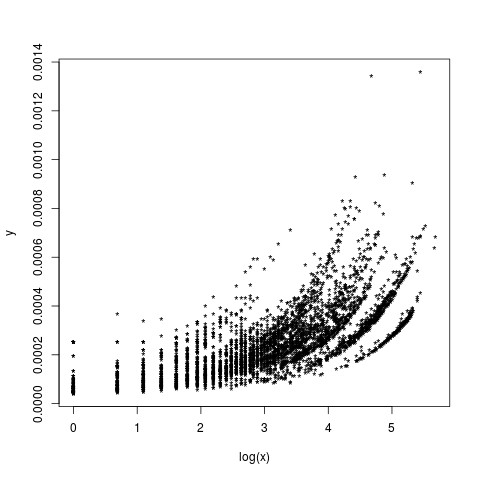
\includegraphics[scale=0.45]{img/fb_grado-pr}
\end{minipage}
\end{figure} 


\begin{figure}[h!] 
\centering 
\begin{minipage}[b]{0.4\textwidth}
	\caption{Barabasi}
	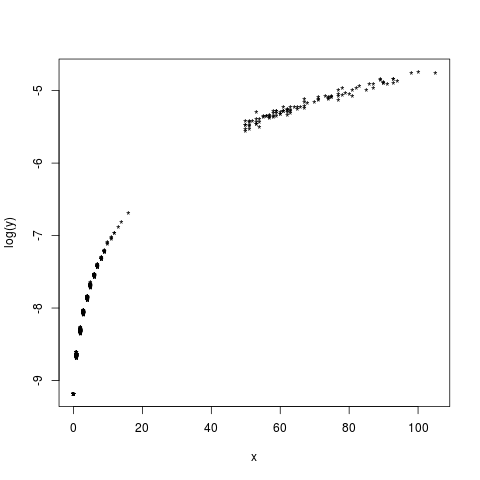
\includegraphics[scale=0.45]{img/barabasi_grado-pr}
\end{minipage}
\hfill
\begin{minipage}[b]{0.4\textwidth}
	\caption{Erdos}
	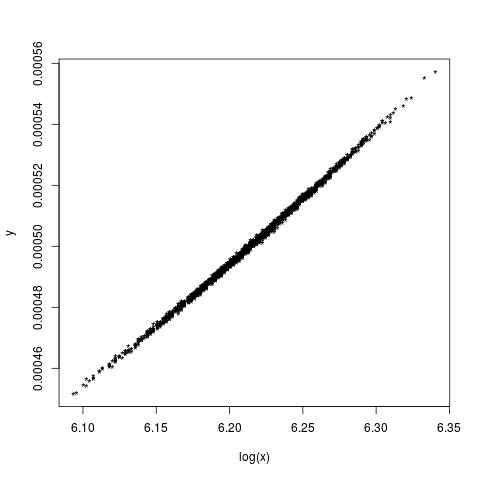
\includegraphics[scale=0.45]{img/erdos_grado-pr}
\end{minipage}
\end{figure} 

\newpage
\subsection{Representación gráfica del grado frente al betweeness }


\begin{figure}[h!] 
\centering 
\begin{minipage}[b]{0.4\textwidth}
	\caption{small1}
	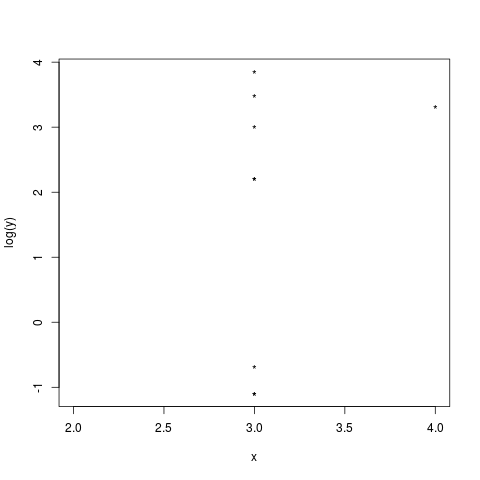
\includegraphics[scale=0.45]{img/small1_grado-betweeness}
\end{minipage}
\hfill
\begin{minipage}[b]{0.4\textwidth}
	\caption{small2}
	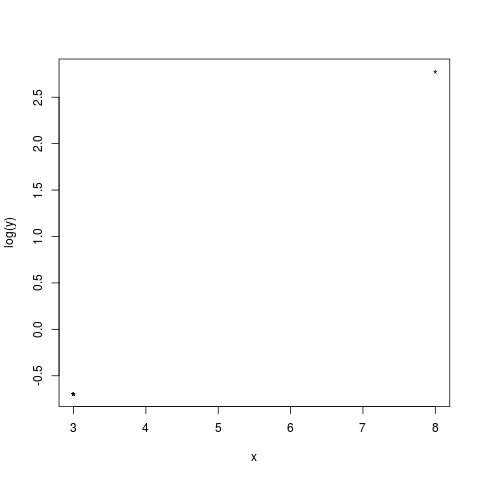
\includegraphics[scale=0.45]{img/small2_grado-betweeness}
\end{minipage}
\end{figure} 


\begin{figure}[h!] 
\centering 
\begin{minipage}[b]{0.4\textwidth}
	\caption{Twitter}
	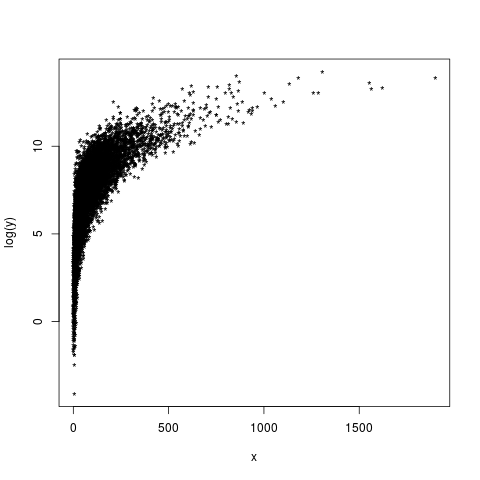
\includegraphics[scale=0.45]{img/twitter_grado-betweeness}
\end{minipage}
\hfill
\begin{minipage}[b]{0.4\textwidth}
	\caption{Facebook}
	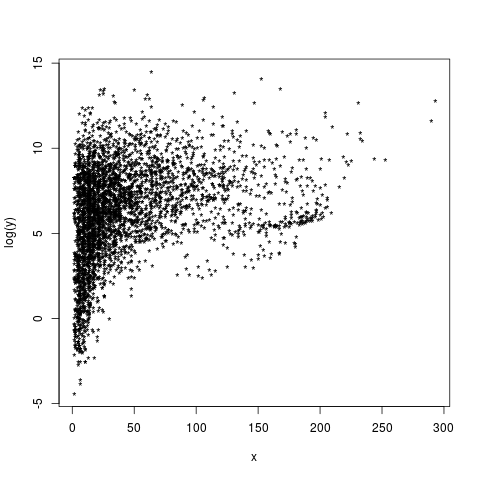
\includegraphics[scale=0.45]{img/fb_grado-betweeness}
\end{minipage}
\end{figure} 


\begin{figure}[h!] 
\centering 
\begin{minipage}[b]{0.4\textwidth}
	\caption{Barabasi}
	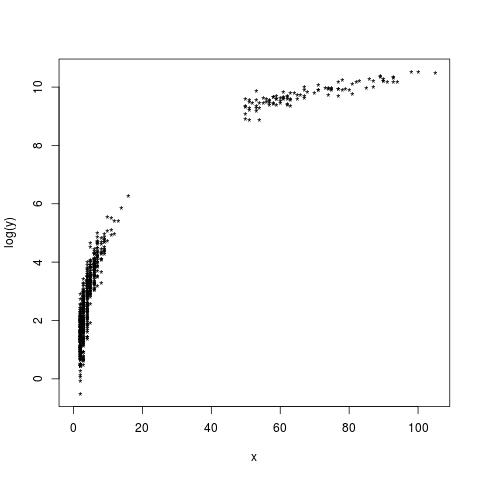
\includegraphics[scale=0.45]{img/barabasi_grado-betweeness}
\end{minipage}
\hfill
\begin{minipage}[b]{0.4\textwidth}
	\caption{Erdos}
	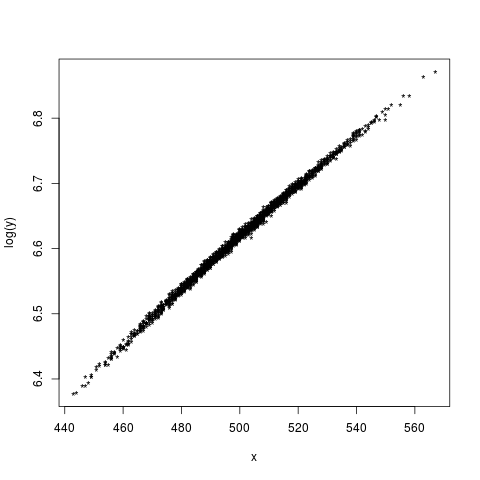
\includegraphics[scale=0.45]{img/erdos_grado-betweeness}
\end{minipage}
\end{figure} 
\end{document}
